\section{SNS Full Analysis}

This document puts forth a proposal for a full Shutdown Dose Rate analysis
of the SNS model using the mesh workflow implementation.
The setup proposed is based on \cite{SNS2018}.

\subsection{Full Transport}
For this transport step the full SNS geometry shown in Figure
\ref{fig:sns_full_geom} will be used.
The neutron flux for the less than
20 MeV (or a threshold that is appropriate) will be collected in a
uniformly distributed Cartesian mesh. A Cartesian mesh with same
dimensions can be used to collect the nuclide production rates. 
Both Cartesian meshes would cover the entire target module shown in Figure
\ref{fig:sns_target}.

\begin{figure}[ht!]
	\centering
	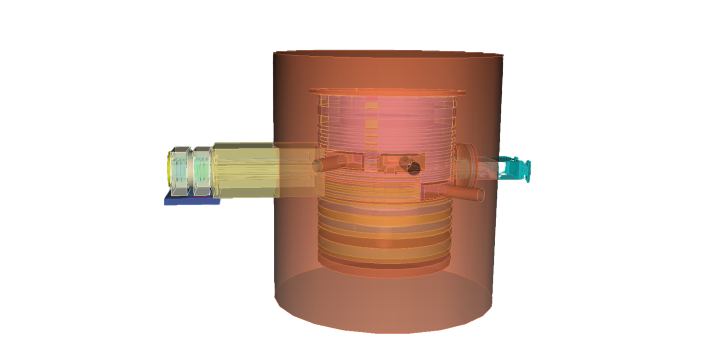
\includegraphics[scale=0.3,trim={3cm 0.5cm 4.5cm 1cm},clip]{figs/SNS_full.png}
	\caption{Full SNS geometry}
	\label{fig:sns_full_geom}
\end{figure}

\begin{figure}[ht!]
	\centering
	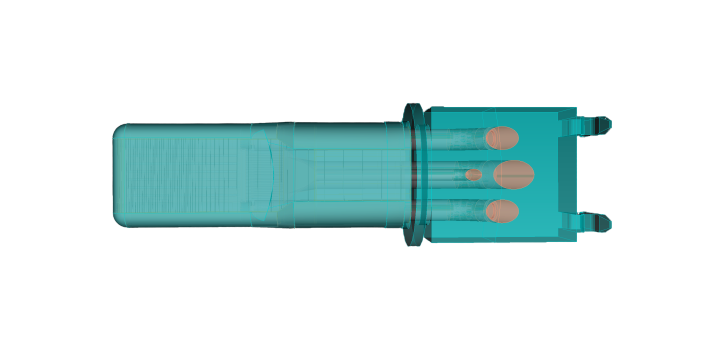
\includegraphics[scale=0.3,trim={3cm 0.5cm 4.5cm 1cm},clip]{figs/SNS_target.png}
	\caption{Target module geometry}
	\label{fig:sns_target}
\end{figure}
In the current CAD geometry the target module consist of four geometric
volumes: mercury, steel, water, and a helium volume.
The water and helium volumes are small and located in between the steel
and mercury volumes.

\subsection{Activation}
The activation geometry will be the target module
(Figure \ref{fig:sns_full_geom}).
From previous papers I have found
that in order to simulate the drainage of the mercury and cooling water
a density of 1.253e-4 $g/cm^{3}$ should be used
for the mercury \cite{SNS2018}.

Photon emission densities will be collected for each mesh
volume element for an irradiation schedule yet to be determined.

\textbf{Question: Is there
an irradiation scenario that simulates realistic irradiation times
that can be used here?}

\subsection{Photon transport}
The geometry for the photon transport  will consist of the target module
with low density mercury
and a set of detectors. The detectors can be placed at the surface
of the geometry and at some distance. Figure \ref{fig:target_detectors} shows an example
of the detector placements at the surface and 30 cm away. These are based
in the work done by \cite{SNS2018}.

\begin{figure}[ht!]
	\centering
	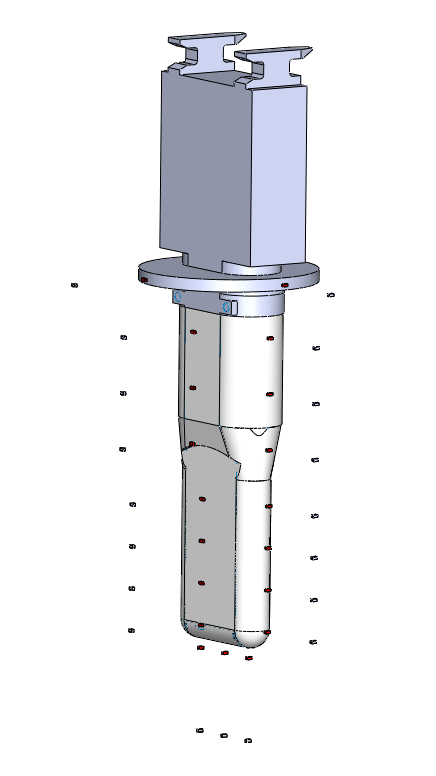
\includegraphics[scale=0.3,trim={0.5cm 0.5cm 0.5cm 0.5cm},clip]{figs/target_detectors.png}
	\caption{Target module and detectors}
	\label{fig:target_detectors}
\end{figure}

The photon source will be a mesh photon source obtained from the activation
calculation. A Cartesian mesh can be used to collect photon flux and the dose
obtained by using flux-to-dose conversion factors. 

\textbf{Question: Some previous papers mention specific
SNS flux-to-dose conversion factors that can be used for this problem. Are these
available for use?}

